\scanpage{65}
% top, two brackets over the three symbols
\figure{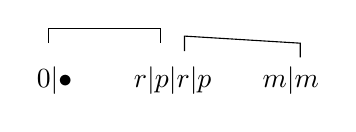
\begin{tikzpicture}[x=1cm,y=1cm]
\node at (0,0) {$\unsure{0|\bullet}$};
\node at (1.5,0) {$\unsure{r|p|\mathfrak r|\mathfrak p}$};
\node at (3,0) {$\unsure{m|\mathfrak m}$};
\draw (-.08,.48)--(-.08,.67)--(1.35,.67)--(1.35,.48);
\draw (1.65,.38)--(1.65,.57)--(3.12,.48)--(3.12,.3);
\end{tikzpicture}}
\[
\widehat A_r\otimes_A K\qquad \widehat{\widehat A\otimes A_r}
\]
\[
\deleted{\widehat{A/r^nA}\otimes A}\qquad \deleted{A_r}\qquad \deleted{A/r^nA}
\]
\[
A/m=\deleted{\unsure{k}} {\unsure{B|\mathscr B}}_0=L_0
\]
\[
\begin{aligned}
\widehat{A/r}&=B_1\subset L_1=\text{\unsure{anneau total des}}\\
&\qquad\text{\unsure{fractions de}}\quad\widehat{A/r}=B_1,\\
&=\unsure{\widehat{A/r}|\widehat A_r}\otimes_A A_r/rA_r
\end{aligned}
\]
\margin{$\varprojlim L_1$}
\figure{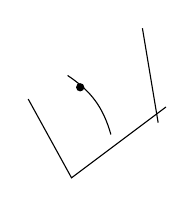
\begin{tikzpicture}
\draw (0,.7)--(.55,-.3)--(1.75,.6); \draw (1.45,1.6)--(1.65,.4);
\draw (.5,1) .. controls (.8,.8) and (.95,.6) .. (1.05,.25);
\fill (.66,.85) circle(1.5pt);
\end{tikzpicture}}
\figure{\begin{tikzpicture}[x=1cm,y=1cm]
\node at (0,0) {$A$};\node at (2,0) {${\unsure{p|\mathfrak p}}_1$};
\node at (2.75,0) {$\supset$};\node at (3.5,0) {$p_2$};
\node at (4.25,0) {$\supset$};\node at (5,0) {$\cdots$};
\node at (5.75,0) {$\supset$};\node at (6.5,0) {$p_n$};
\draw (2,.35)--(2,.52)--(3.25,.52)--(3.25,.35);
\draw (5.65,.35)--(5.65,.52)--(6.55,.52)--(6.55,.35);
\node at (2.65,.8) {$1$};\node at (6.1,.8) {$1$};
\end{tikzpicture}}
\[
A_{[p_1,p_2,\ldots,p_n]}
\]
\unsure{définition par récurrence sur} $n\geq1$

\margin{$A\unsure{\longrightarrow|-}\widehat A_p$ \unsure{anneau local complet}}
\[
A_{\unsure{\{p\}|[p]}}=\widehat A_p
\]
si $n=1$ ; c'est un \deleted{\unsure{filtre|fibré}} \inserted{\unsure{anneau}} local noeth. \inserted{\unsure{sur $A$}} et \unsure{complet} et une \unsure{algèbre} sur $A$.
\[
\begin{gathered}
A_{p,\unsure{q|\mathfrak q}}=\deleted{\unsure{\prod}}\varprojlim_n\widehat A_p\otimes_A A_q/q^nA_q
\qquad A_{[p_1\,\text{--}\,p_{n-1}]}\\
p\supset q\\
\widehat{A_p/qA_p}\quad\otimes
\end{gathered}
\]
\unsure{déjà défini}, c'est un \unsure{anneau} local \unsure{noethérien} \unsure{séparé} et \unsure{complet}, et une \unsure{algèbre} sur $A$.

\unsure{anneau semi-local complet} dont le \deleted{\unsure{corps}} \inserted{\unsure{anneau}} résiduel $\unsure{k|\kappa}(p,q)$ est l'anneau \unsure{tot.l|total} des fractions de
\[
\widehat{A_p/qA_p}=\widehat A_p/q\widehat A_p
\]
(\unsure{complété d'un anneau} local \unsure{intègre} noeth. de dim $1$)
% archive sheet number: 64
